\documentclass[a4paper, 12pt]{article}

\usepackage{mathtools}
\usepackage{graphicx}
\usepackage{amsmath}

\usepackage{caption}
\usepackage{subcaption}

\usepackage[margin=1in, bottom=0.5in, includefoot]{geometry}

\usepackage{fancyhdr}
\pagestyle{fancy}
\fancyhead{}
\fancyfoot{}
\fancyfoot[R]{\thepage}
\renewcommand{\headrulewidth}{0pt}

\graphicspath{{./images/}}

\begin{document}

\begin{titlepage}
	\begin{center}
	
\includegraphics{logo}\\
	\large{\textbf{TRIBHUVAN UNIVERSITY\\ INSTITUTE OF ENGINEERING \\ PULCHOWK CAMPUS}}\\
	\large{LAB REPORT}\\
	
	\begin{picture}(50,250)
		\put(0,--25){\line(0,1){150}}
		\put(25,-25){\line(0,1){250}}
		\put(50,25){\line(0,1){150}}
	\end{picture}
	\end{center}
	\vspace{1cm}
	\begin{minipage}{2.5in}

    	Lab No: \\
    	Experiment Date: 2020-5-26\\
    	Submission Date: 2020-6-7\\

    	\textbf{\underline{Submitted By:}}\\
    	Name: Suban Shrestha \\
    	Roll No: 076BCT082 \\
    	Group: CD(D)
	\end{minipage}
	\hfill
	\begin{minipage}{1.3in}
    	\textbf{\underline{Submitted To:}}\\
    	Department of Electronics and Communications Enginnering
	\end{minipage}
\end{titlepage}

{\LARGE{\textbf{Verification of DeMorgan's Laws and Familiarization with NAND and NOR Gates}}}

\section{Objectives}
\begin{enumerate}
  \item
    To learn, understand and verify DeMorgan's Laws.
  \item
    To get familiarized with NAND and NOR Gates, universal gates.
  \item
    To construct various gates using universal gates.
\end{enumerate}
\section{Materials Required}
\begin{enumerate}
  \item
    Universal Gates(NAND and NOR gates).
  \item
    Basic Logic Gates(AND, OR and NOT gates).
  \item
    For computer simulation, a computer with simulation software.
\end{enumerate}

\pagebreak
\section{Theory}
\subsection{DeMorgan's Law}
DeMorgan's Theoreams are a set of laws developed from boolean expressions for AND, OR and NOT using two input variables, A and B. The two theorems allow the input variables to be negated and be converted from one boolean function to the opposite form. It can also be used to relate negative logic with positive logic.

\subsubsection{DeMorgan's First Law}
DeMorgan's First theorem proves that when two input variables are AND'ed and negated, the are equivalent to the OR of the complement of the individual variables. Thus the equivalent of the NAND function will be a negative-OR function.

\begin{center}
  $(A . B)' = A' + B'$
\end{center} 

\begin{center}
  \begin{tabular}{|c|c|c|c|c|c|c|}
    \hline
    \multicolumn{2}{|c|}{Inputs}& \multicolumn{5}{|c|}{Outputs}  \\
    \hline
    A & B & $A.B$ & A' & B' & $(A.B)'$ & $A' + B'$ \\
    \hline
    0 & 0 & 0 & 1 & 1 & 1 & 1\\
    0 & 1 & 0 & 1 & 0 & 1 & 1\\
    1 & 0 & 0 & 0 & 1 & 1 & 1\\
    1 & 1 & 1 & 0 & 0 & 0 & 0\\
    \hline
  \end{tabular}
  \captionof{table}{Truth Table}
  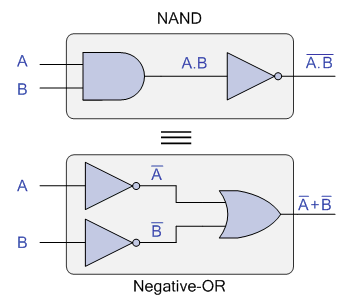
\includegraphics{demorgan-first}
  \captionof{figure}{Implementation using Logic Gates}
\end{center}

\subsubsection{DeMorgan's Second Law}
DeMorgan's Second theorem proves that when two input variables are OR'ed and negated, the equivalent to the AND of the complement of the individual variables. Thus the equivalent of the NOR function will be a negative-AND function.
\begin{center}
  $(A + B)' = A' . B'$
\end{center} 

\begin{center}
  \begin{tabular}{|c|c|c|c|c|c|c|}
    \hline
    \multicolumn{2}{|c|}{Inputs}& \multicolumn{5}{|c|}{Outputs}  \\
    \hline
    A & B & $A+B$ & A' & B' & $(A+B)'$ & $A' . B'$ \\
    \hline
    0 & 0 & 0 & 1 & 1 & 1 & 1\\
    0 & 1 & 1 & 1 & 0 & 0 & 0\\
    1 & 0 & 1 & 0 & 1 & 0 & 0\\
    1 & 1 & 1 & 0 & 0 & 0 & 0\\
    \hline
  \end{tabular}
  \captionof{table}{Truth Table}
  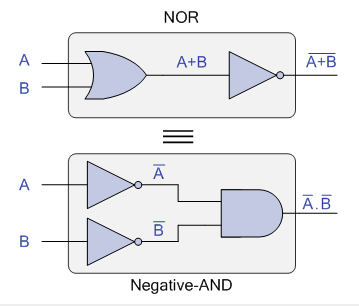
\includegraphics{demorgan-second}
  \captionof{figure}{Implementation using Logic Gates}

\end{center}
\subsection{Universal Gates}
The gates NAND and NOR are knows as universal gates. These gates can be used to create the logic of all ther other gates. Because of this, these are known as universal gates. Using only one type of gate is more efficient in building large scale devices and thus they are used.

\section{Lab}
\subsection{DeMorgan's Laws}
The circuits below were constructed for the verification of DeMorgan's laws. Various inputs were provided and the truth table was verified.

\begin{figure}[h]
  \centering
  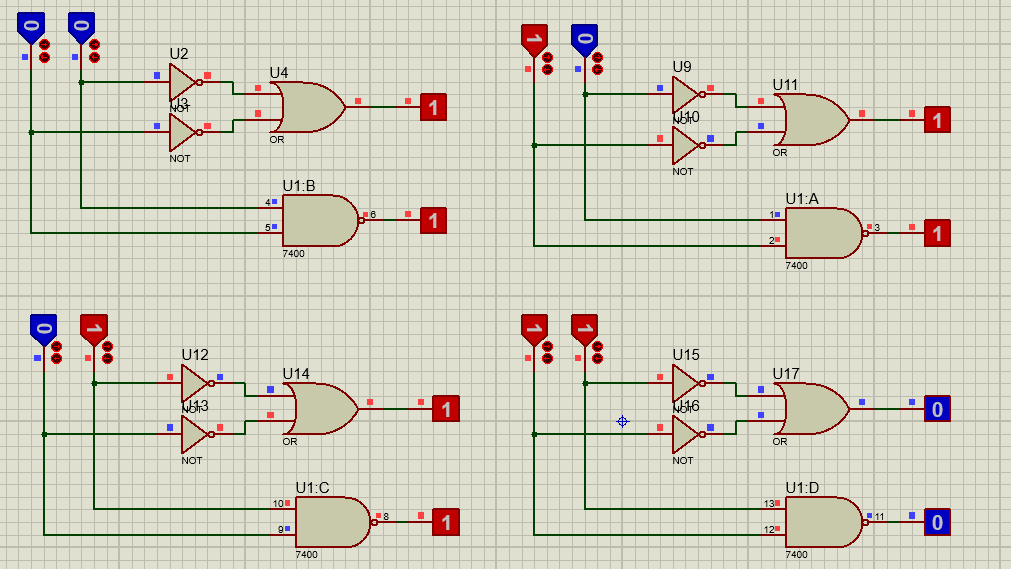
\includegraphics[scale=0.55]{deMorgan1}
  \caption{DeMorgan's First Law}
\end{figure} 

\begin{center}
  \begin{tabular}{|c|c|c|c|}
    \hline
    A & B & $(A.B)'$ & $A' + B'$ \\
    \hline
    0 & 0 & 1 & 1 \\
    0 & 1 & 1 & 1 \\
    1 & 0 & 1 & 1 \\
    1 & 1 & 0 & 0 \\
    \hline
  \end{tabular}
  \captionof{table}{Truth Table verification of DeMorgan's First Law}
\end{center}
Thus DeMorgan's first law was verified

\pagebreak

Simillarly Another circuit was constructed to verify DeMorgan's Second Law.
\begin{figure}[h]
  \centering
  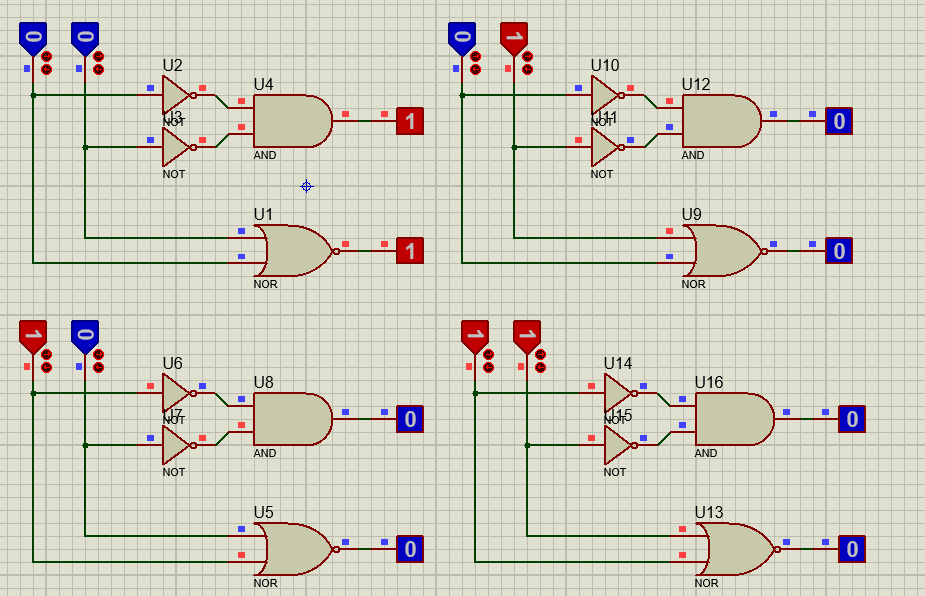
\includegraphics[scale=0.6]{deMorgan2.png}
  \caption{DeMorgan's Second Law}
\end{figure} 


\begin{center}
  \begin{tabular}{|c|c|c|c|}
    \hline
    A & B & $(A+B)'$ & $A' . B'$ \\
    \hline
    0 & 0 & 1 & 1 \\
    0 & 1 & 0 & 0 \\
    1 & 0 & 0 & 0 \\
    1 & 1 & 0 & 0 \\
    \hline
  \end{tabular}
  \captionof{table}{Truth Table verification of DeMorgan's Second Law}
\end{center}
Thus DeMorgan's second law was verified.
\pagebreak
  
\subsection{Construction of Basic Gates from Universal Gates}
\subsubsection{AND from NAND Gate}
\begin{center}
  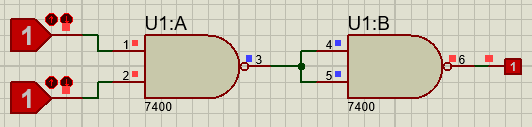
\includegraphics[scale=0.75]{nand-and}
\end{center}
\textbf{Boolean Logic}
\begin{equation} 
\begin{split}
  Y & = ((A.B)')' \\
    & = A.B \\
\end{split}
\end{equation}

\subsubsection{NOT from NAND Gate}
\begin{center}
  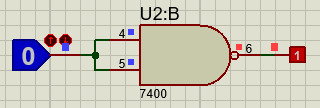
\includegraphics[scale=0.75]{nand-not}
\end{center}
\textbf{Boolean Logic}
\begin{equation} 
\begin{split}
  Y & = (A.A)'  \\
    & = A'  \\
\end{split}
\end{equation}

\subsubsection{OR from NAND Gate}
\begin{center}
  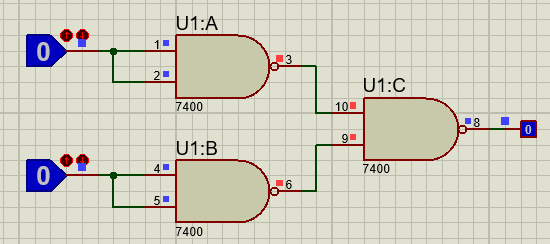
\includegraphics[scale=0.75]{nand-or}
\end{center}
\textbf{Boolean Logic}
\begin{equation} 
\begin{split}
  Y & = (A' . B')' \\
  Y & = (A+B)'' \\
    & = A+B\\
\end{split}
\end{equation}

\subsubsection{AND from NOR Gate}
\begin{center}
  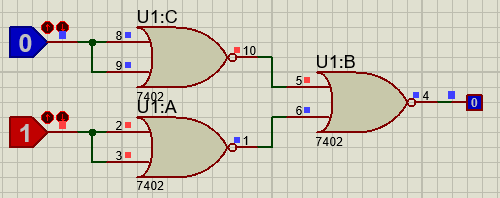
\includegraphics[scale=0.75]{nor-and}
\end{center}
\textbf{Boolean Logic}
\begin{equation} 
\begin{split}
  Y & = (A' + B')'\\ 
    & = ((A.B)')' \\
    & = A.B \\
\end{split}
\end{equation}

\subsubsection{NOT from NOR Gate}
\begin{center}
  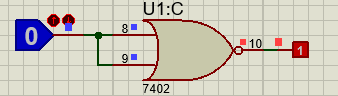
\includegraphics[scale=0.75]{nor-not}
\end{center}
\textbf{Boolean Logic}
\begin{equation}
\begin{split}
  Y & = (A+A)'  \\
    & = A'  \\
\end{split}
\end{equation}

\subsubsection{OR from NOR Gate}
\begin{center}
  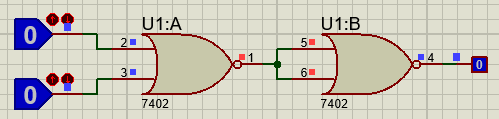
\includegraphics[scale=0.75]{nor-or}
\end{center}
\textbf{Boolean Logic}
\begin{equation} 
\begin{split}
  Y & = ((A+B)')' \\
    & = (A+B)'' \\
    & = A+B\\
\end{split}
\end{equation}

\pagebreak
\subsection{XOR and XNOR Gates}

\subsubsection{XOR from NAND Gate}
\begin{center}
  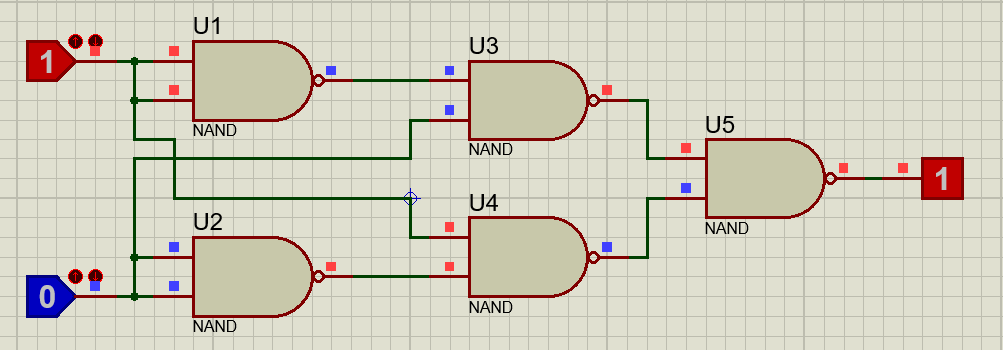
\includegraphics[scale=0.5]{nand-xor}
\end{center}
\textbf{Boolean Logic}
\begin{equation} 
\begin{split}
  Y & = AB' + A'B \\
    & = (AB' + A'B)'' \\
    & = ((AB')' . (A'B)')' \\
\end{split}
\end{equation}

\subsubsection{XNOR from NAND Gate}
\begin{center}
  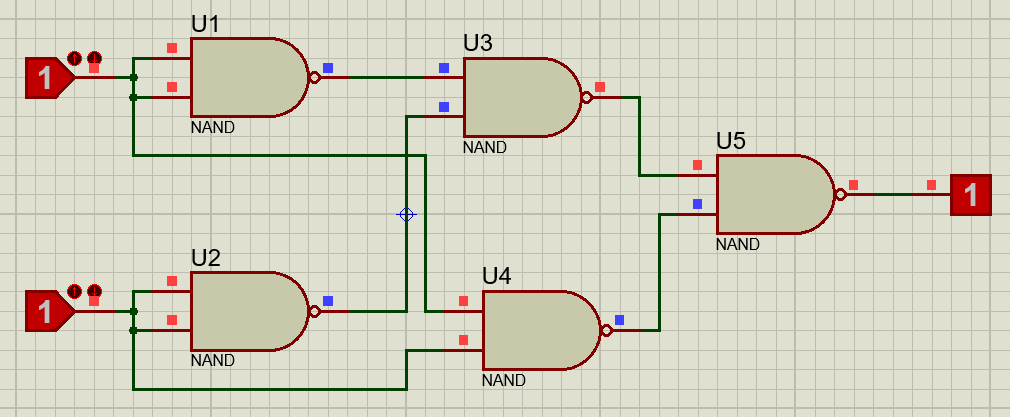
\includegraphics[scale=0.5]{nand-xnor}
\end{center}
\textbf{Boolean Logic}
\begin{equation} 
\begin{split}
  Y & = AB + A'B' \\
    & = (AB + A'B')'' \\
    & = ((AB)' . (A'B')')' \\
\end{split}
\end{equation}

\subsubsection{XOR from NOR Gate}
\begin{center}
  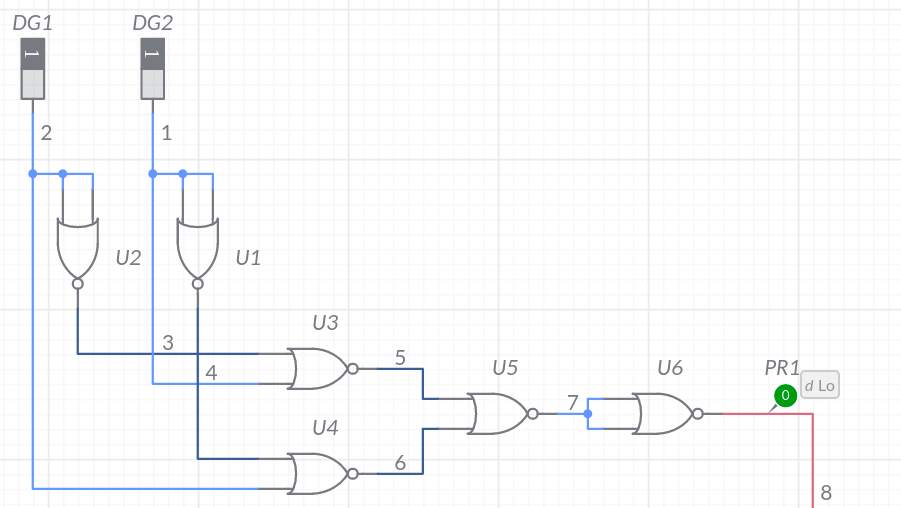
\includegraphics[scale=0.5]{nor-xor}
\end{center}
\textbf{Boolean Logic}
\begin{equation} \label{eq1}
\begin{split}
  Y & = (AB' + A'B) \\
    & = (AB')'' + (A'B)''  \\
    & = (A' + B)' + (A + B')' \\
    & = ((A' + B)' + (A + B')')'' \\
\end{split}
\end{equation}

\subsubsection{XNOR from NOR Gate}
\begin{center}
  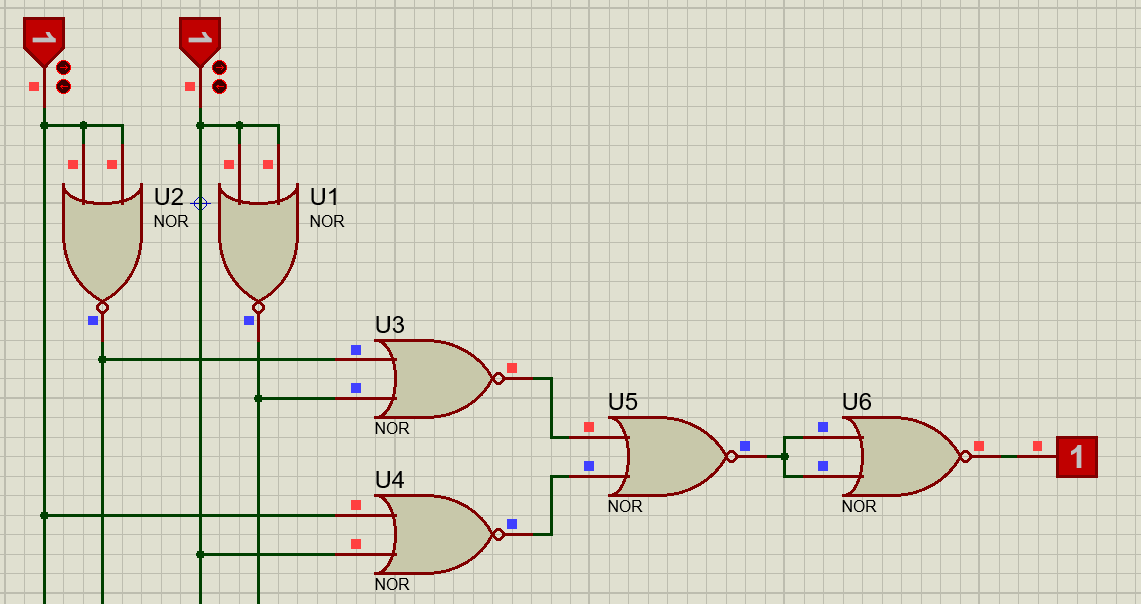
\includegraphics[scale=0.5]{nor-xnor}
\end{center}
\textbf{Boolean Logic}
\begin{equation} 
\begin{split}
  Y & = AB + A'B'\\
    & = (AB)'' + (A'B')'' \\
    & = (A' + B')' + (A + B)' \\
    & = ((A' + B')' + (A + B)')'' \\
\end{split}
\end{equation}

\section{Discussion}
In this way, DeMorgan's laws were studied and verified using a truth table and circuit. A through understanding of the universal gates was also gained. The universal gates were then used to make other gates like AND, OR, NOT, XOR and XNOR, by the use of boolean algebra and DeMorgan's laws. The working of Negative OR and Negative AND gate was also gained. All of the simulation was done using a simulating software.

\section{Conclusion}
Thus, various circuits were constructed by the use of boolean algebra and DeMorgan's Laws, and were verified in the simulation.
A through understanding of the Demorgan's laws and Universal Gates was obtained through the use of simulating software.
\end{document}

